\section{Prior Deepsense Methods}
The Deepsense 6G dataset is a real-world multi-modal dataset that provides researchers a comprehensive dataset for multi-modal sensing and communication data. The dataset provides the world's first large-scale real-world sensing and communication reprository of over a million data points, with over 30 different scenarios that target multiple applications. The team that provided the DeepSense 6G dataset aims to provide a platform that encourages the development of machine learning solutions for applications in communication systems, through a variety of multi-modal sensor technologies. There are various tasks that are supported by the dataset as well, ranging from \textit{Sensing Aided Beam Prediction} to \textit{Future Blockage Prediction}, with each task supported by a diverse set of sensing modalities. The dataset provides multiple input modalities such as GPS, Camera, Radar, and LiDAR sensing modalities aimed to enhance the breadth of the dataset for various applications. In addition to the various data points, test benches, and scenarios, the Deepsense team provides a wide array of papers, code bases, and techniques for solving problems relevant to the dataset. The inception of the DeepSense 6G dataset has marked a significant milestone in fostering research within the field of communications, particularly in scenarios requiring multi-modal sensor integration. Before the introduction of datasets like DeepSense 6G, researchers encountered substantial challenges, predominantly due to the lack of access to large-scale, realistic datasets that reflect the complexity and variety of real-world environments. \cite{alkhateeb2023deepsense}

Traditional methods for beam management often rely on exhaustive beam search techniques, which often have drawbacks in high overhead and an intractible search space. Leveraging a large-scale dataset Machine Learning frameworks are viable alternative to traditional datascience techniques as outlined in the paper, \textit{Computer Vision Aided Beam Tracking in a Real-World Millimeter Wave Deployment}. In this work the authors propose to utilize temporal visual sensing information to predict the optimal beam, as defined as the highest beamforming gain through the use of an Encoder-Decoder network. The paper presents an innovative machine learning (ML) model for beam tracking optimization in mmWave communication systems, in which a base station is equipped with an antenna array and an RGB camera to assist mobile users. The proposed model leverages visual sensing information alongside pre-defined beamforming codebooks to predict optimal future beams using an encoder-decoder architecture leveraging Recurrent Neural Networks (RNNs). The vision-aided approach demonstrates promise over the traditional methods by leveraging existing feature extraction networks to enhance beamforming gain and communication performance. \cite{jiang2022computer} The paper underscores the effectiveness of machine learning-based and vision-aided beam tracking in mmWave communications. This approach shows that it is possible to achieve a high level of accuracy for narrowing the beam search to top-5 accuracy with a precision of 99.37 percent for the next beam by observing previous time-steps on a single scenario.

\begin{figure}[h!]
  \centering
  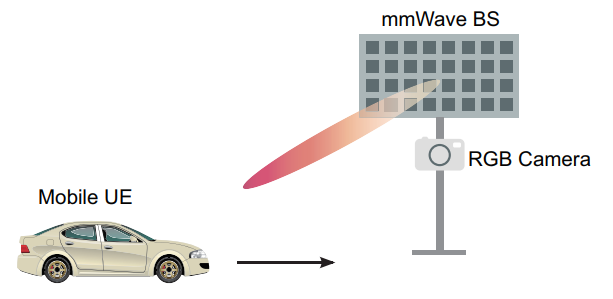
\includegraphics[width=0.5\textwidth]{Images/Literature_Review/jiang2022computer_paper.png}
  \caption{The considered system model leveraged to design a computer vision aided Beam Tracking system \cite{jiang2022computer}.}
  \label{fig:my_label}
\end{figure}

The paper's focus on next beam prediction presents limited scope, and does not take into account the some of the deeper challenges often faced in wireless communication systems by limiting it's evaluation to a single scenario. In turn the paper fails to consider the variability of real-world environments. The omission of additional sensing modalities such as radar, GPS, or other sensing inputs might limit the system's capabilites in Non-Line of Sight conditions (NLOS), where additional information might be crucial. Other methods delve into the usage of position-aided beam prediction aiming to evaluate the practicality of GPS guided predictions. In the paper \textit{Position-aided Beam Prediction in the Real World: How Useful GPS Locations Actually Are?}, the authors propose three machine learning solutions for position-aided mmWave beam prediction. They evaluate multiple methods using a Lookup Table, K-Nearest Neighbors, and a fully connected Neural network against three different scenarios. The paper reveals that the Neural Network generally outperforms both the lookup table and K-Nearest Neighbors in top-1 predictions across various scenarios due to the ability of the Neural Network to generalize better and utilize more information from training samples. They do note that factors such as input noise and label noise degrades performance and necessitates alternate metrics such as power loss, but the paper outlines the practical implications of using position data for beam alignment. Additionally, the authors point out that utilizing GPS positions can provide significant savings for the overhead of beam search in a code book that contains 64 unique codes. \cite{morais2023position}. There are several drawbacks to the use of GPS for beam alignment and some of these challenges include susceptibility to noisy inputs, latency issues, and environmental constraints, which lead the authors to suggest techniques that do not solely rely on GPS based methods. 

Location-aware methods offer a practical approach but come with limitations such as latency issues, environmental blockages, and noisy inputs. Works by the DeepSense team explore the efficacy of using Radar Aided Beam Prediction in the paper \textit{Radar Aided 6G Beam Prediction: Deep Learning Algorithms and Real-World Demonstration}. The team proposes a novel radar-aided deep learning framework to map radar samples to the optimal beam predictions. The framework leverages preprocessing of the radar samples into feature maps such as range, angle, and velocity maps using Fast Fourier Transforms (FFTs) and then employ a deep neural network subsequently to learn the mapping from the features to optimal beamforming predictions. The network is designed to be a relatively simple deep network comprosing of convolutional and fully-connected layers utilizing the rectified linear unit (ReLU) non-linear activation functions. The final layer of the network maps a hidden-layer to the designed beam code book size of 64 positions in which the objective function utilizes cross-entropy loss for predicting the optimal beam. The promise for utilizing relatively simple deep learning networks and demonstrates the capabilities of the approach showing how a the model can acheive around 90 percent for top-5 accuracy. This research underscores the potential for utilizing radar for inferring beam prediction with the radar modality. \cite{demirhan2022radar} 

\begin{figure}[h!]
  \centering
  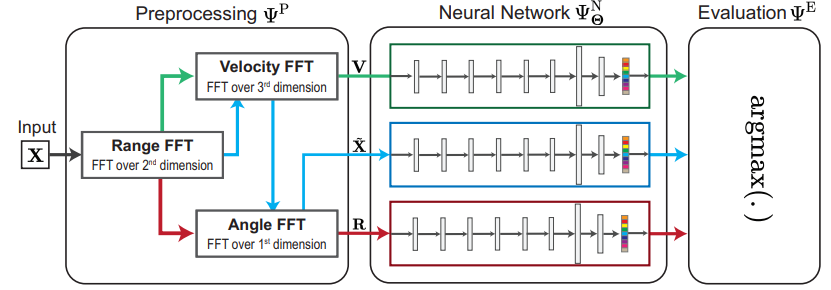
\includegraphics[width=0.5\textwidth]{Images/Literature_Review/demirhan2022radar_architecture.png}
  \caption{The considered architecture leveraged implemented in the radar aided Beam tracking paper. \cite{jiang2022computer}.}
  \label{fig:my_label}
\end{figure}

In addition to radar, vision, or position based sensing methods, other modalities like LiDAR (Light Detection and Ranging) can contibute to the diversification of environmental perception. \textit{LiDAR Aided Future Beam Prediction in Real-World Millimeter Wave V2I Communications} explores the effectiveness of utilizing LiDAR in the Beam prediction and reduction tasks. The authors argue that vision-aided methods might fall short in low light conditions, and may cause privacy concerns when it comes to positional information of the end user. The paper investigates utilizing LiDAR for mmWave beam prediction and tracking tasks, which in turn shows promising results in predicting optimal beam at 95 percent for top 5 accuracy.   


% Need to transition into accross scenario review (Scene Generalization) -- Talk about the papers from the competition


% Review of Transformers and why is it relevant, Attention is All you need, 

% Discuss VLMs starting at CLIP and ending with foundational models such as Florence, SAM, SEEM etc

% Go into High level Applications for LLMs and VLMs such as RAG







% \section{Self-Supervised Methods}
% % Some topics to discuss in self-supervised learning
% % Pseudo Labels, Pretext tasks, Positive/Negative Pairs, Augmnentations
% % General Algorithms for SSL i.e. Contrastive Learning, DINO, MoCo, SMoG...

% Multimodal methods require expensive human annotation for effective training, and makes scaling these multimodal network difficult. \cite{zong2023self} Self-Supervised methods has shown promise to take unlabeled data and address the issue of the manual annotation bottleneck. \cite{zong2023self} Self-supervised learning can be separated into different distinct methods based on the objective of the learning task, such as contrastive learning, cluster analysis, and cross modal learning. The benefits of using self-supervised methods have shown to enable models in learning more generalize and robust representations of data since the learning objective is not limited to annotations.


% \section{Multimodal Self Supervised Methods}
% A self-supervised multimodal survey \cite{zong2023self} address the concepts around self-supervised multimodal learning, which is shown to significantly enhance the capability and power of multimodal models. The survey begins with how to conduct multimodal representation learning without labels, how to fuse different modalities, and how to learning from partially or completely unaligned multimodal data. \cite{zong2023self} Self-Supervised multimodal fusion can be achieved in two ways: multimodal pretraining with a fusion architecture or amalgamation of independently pre-trained unimodels (i.e. "stitching") \cite{zong2023self} 


% \subsection{Learning Paradigms}

% \subsection{Constrastive Learning}
% Contrastive methods typically use corresponding samples from different modalities as positive example pairs and noncorresponding samples as negative pairs. These pairs are then used to train a model to accurately distinguish positive and negative pairs using contrastive training objectives. The general form of Contrastive Learning is shown below


% Contrastive Multiview Coding \cite{zong2023self} [23] is one of the earliest works to explore Contrastive Learning in a multimodal setting and aims to maximize the view between representations of different views in the same scene. AVTS \cite{zong2023self}[43] considers temporally synchronized audio-video pairs as positives and utilizeis cirriculum Learning to gradually learn hard negatives. MultiModal Versatile Networks \cite{zong2023self}[45] and Video-Audio-Text transformer (VATT) \cite{zong2023self}[46] are also examples that can learn mutual information among vision, audio, and text. Contrastive Learning has also shown great potential for scaling with CLIP \cite{zong2023self}[21] and this paradigm has been applied to other domains such as AudioCLIP \cite{zong2023self}[47], VideoCLIP \cite{zong2023self}[48], CLIP4CLIP \cite{zong2023self}[49], and pointCLIP \cite{zong2023self}[50]. Techniques such as CrossCLR, SLIP \cite{zong2023self}[54], and COOKIE \cite{zong2023self}[55] apply intra-modality learning alongside cross modal learning to help preserve proximity in the joint embedding space. \cite{zong2023self}[56]. The intramodal methodology does not always improve performance due to the ease of pretext tasks as shown in AVID \cite{zong2023self}[58].